\chapter{Stochastic Approximation}

This chapter covers some of the basic results in the theory of stochastic approximation and in doing so provides some applications of discrete time martingale theory and weak convergence theory to optimization problems.  The statement of the stochastic approximation problem that one often encounters is so abstract and general that it can be difficult to understand how it could be relevant to any particular problem.  Indeed it is common to see stochastic approximation defined as the study of discrete time stochastic processes of the form 
\begin{align*}
\theta_{n+1} &= \theta_n + \epsilon_n Y_n
\end{align*} 
where $Y_n$ is a random vector.

To motivate the form of the problem statement, let us tie this into the problem of optimization specifically gradient descent.  Given a function $f$ we have a globally convergent algorithm for minimization given by $x_{n+1} = x_n - \alpha_n \nabla f(x_n)$ where $\alpha_n$ is a sequence of real numbers that satisfies Armijo conditions.  Now suppose that we don't have the ability to measure $-\nabla f(x_n)$ exactly but that we have some noise corrupted  version thereof.  If we call the observed approximate gradient $Y_n$, then the gradient descent algorithm has the form of a stochastic approximation problem and we can ask whether we still have convergence in a appropriate stochastic sense (e.g. almost sure).  In line with this specific case, we often think of the process $Y_n$ as being a sequence of observations and though it doesn't have any real mathematical meaning, we shall use the terminology in what follows.

As we've mentioned in our discussion of optimization, in practice constrained optimization is at least as important as unconstrained optimization and therefore we should look for how to incorporate constraints into stochastic approximation.  The way we shall do this at this point is to assume that the sequence $\theta_n$ is constrained to lie in some closed set $F$ and to maintain the constraint at each iteration by a brute force projection (say in $L^2$ norm) onto the set $F$.   Thus in the constrained case we are considering a stochastic process 
\begin{align*}
\theta_{n+1} &= \Pi_F \left[ \theta_n + \epsilon_n Y_n\right ]
\end{align*} 
where $Y_n$ is a random vector and $\Pi_F$ represents projection onto $F$.  It is common to define the projection correction term $Z_n =  \epsilon_n^{-1} \lbrace \Pi_F \left[ \theta_n + \epsilon_n Y_n\right ] -   \theta_n - \epsilon_n Y_n \rbrace$ so that we may write 
\begin{align*}
\theta_{n+1} &= \theta_n + \epsilon_n Y_n + \epsilon_n Z_n
\end{align*} 

In order to discuss the hypotheses that one might need to make on the stochastic process $Y_n$, it is convenient to assume a structural form for $Y_n$.  Let $\mathcal{F}_n = \sigma(\theta_0, Y_j ; j<n)$ be a filtration $\mathcal{F}$.  For our first results we shall assume that there exists functions $g_n$, an $\mathcal{F}$-martingale difference sequence $\delta M_n$ and a stochastic process $\beta_n$ such that $Y_n = g_n(\theta_n) + \delta M_n + \beta_n$.  The reader should think of these terms in the following way.  The term $g_n(\theta_n)$ represents the mean/true value of the process (e.g. the value of the gradient in the steepest descent case), the term $\delta M_n$ represents a noise term and $\beta_n$ represents a bias term in the observation.  The reason why the bias term $\beta_n$ is called out as being different from $g_n(\theta_n)$ is that we shall be assuming that it becomes asymptotically small.

One of the key techniques in proving theorems in stochastic approximation is the ODE method.  The basic idea is that one can view the process $\theta_n$ as a discretization of an ordinary differential equation 
that is described by the conditional means of $Y_n$.  

In many of the proofs we will considering the continuous time limits of discrete time processes.  To do this we be making interpolations of the discrete time processes and want to have recourse to compactness results that will give conditions under which limits exist.  A natural tool for this would be to use the Arzela-Ascoli Theorem for continuous functions or the Skorohod topology versions of that for cadlag functions.  As it turns out neither of these is the exact fit for what we do since we'll be considering cadlag processes that converge to continuous functions and we want uniform convergence on compact sets.  So what we want is a slight extension of Arzela-Ascoli.

We also need a partial converse, namely that a convergence sequence of functions is equicontinuous in the extended sense.
\begin{prop}\label{PartialConverseExtendedArzelaAscoli}Let $f_n : \reals \to \reals^d$ be a sequence of measurable functions that converges to a continuous function with convergence uniform on compact sets, then $f_n$ is equicontinuous in the extended sense.
\end{prop}
\begin{proof}
Let $f$ be the limit of $f_n$.  Pick an $N$ such that $\norm{f_n(0) - f(0)} < 1$ for all $n \geq N$ then it follows that $\norm{f_n(0)} \leq \norm{f_0(0)} \vee \dotsb \vee \norm{f_{N-1}(0)} \vee \norm{f_N(0)} + 1$ for all $n \in \naturals$.  Now let $T > 0$ and $\epsilon > 0$ be given and use the fact that $f$ is uniformly continuous on $[-T,T]$ to pick 
a $\delta > 0$ such that $m(T, f, \delta) < \epsilon/3$.  Now by uniform convergence of $f_n$ to $f$ on $[-T,T]$ we pick $N > 0$ such that $\sup_{-T \leq t \leq T} \norm{f_n(t) - f(t)} < \epsilon/3$ for $n \geq N$.  Thus for $n \geq N$,
\begin{align*}
m(T,f_n,\delta) &= \sup_{\substack{
\abs{s -t} < \delta \\
-T \leq s,t \leq T}} \norm{f_n(s) - f_n(t)} \\
&\leq \sup_{\substack{
\abs{s -t} < \delta \\
-T \leq s,t \leq T}} \norm{f_n(s) - f(s)} + \norm{f(s) - f(t)} + \norm{f_n(t) - f(t)} < \epsilon
\end{align*}
and it follows that $\limsup_{n \to \infty} m(T, f_n, \delta) < \epsilon$ and thus $\lim_{\delta \to 0} \limsup_{n \to \infty} m(T, f_n, \delta) = 0$.
\end{proof}

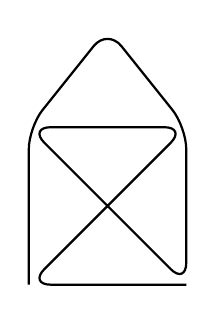
\begin{tikzpicture}
\draw[thick,rounded corners=8pt] (0,0) -- (0,2) --(1,3.25) -- (2,2) -- (2,0) -- (0,2) -- (2,2) -- (0,0) -- (2,0);
\end{tikzpicture}

We shall now assume that we are in the situation of having a constraint set $F$ defined by continuously differentiable function $c_i(x)$ which satisfy the LICQ.  

TODO:  Use the KKT  conditions applied to $\min_{x \in F} \norm{x - (\theta_n + \epsilon_n Y_n)}^2$ to show that $Z_n$ is in the normal cone 


\begin{thm}Suppose we are given a process $Y_n$, a constraint set $F$, a random variable $\theta_0$ and a deterministic sequence $\epsilon_n$.  Define the process 
\begin{align*}
\theta_{n+1} &= \Pi_F \left[\theta_{n} + \epsilon_n Y_n \right]
\end{align*}
and suppose that there are measurable functions $g_n(\theta)$ such that if we write $\cexpectationlong{\theta_0, Y_i; 0 \leq i \leq n-1}{Y_n} = g_n(\theta_n) + \beta_n$ such that
\begin{itemize}
\item[(i)] $\sup_n \expectation{Y_n^2} < \infty$
\item[(ii)] $\epsilon_n$ for $n \in \integers$ is a sequence with $\epsilon_n = 0$ for $n < 0$, $\epsilon_n \geq 0$ for $n \geq 0$, $\lim_{n \to \infty} \epsilon_n = 0$,  $\sum_{n=0}^\infty \epsilon_n = \infty$ and $\sum_{n=0}^\infty \epsilon^2_n < \infty$.  
\item[(iii)] Suppose the $g_n(\theta)$ are uniformly continuous in $n$ and there is a continuous function $\overline{g}(\theta)$ such that for each $\theta \in F$ we have
\begin{align*}
\lim_{n \to \infty} \abs{\sum_{i=n}^{m(t_n+t)} \epsilon_i \lbrace g_i(\theta) - \overline{g}(\theta) \rbrace }&= 0
\end{align*}
\item[(iv)] $\beta_n \toas 0$
\end{itemize}
Then there is a set $A$ of probability zero such that for $\omega \notin A$ the set of functions $\lbrace \theta^n(\omega, \cdot), Z^n(\omega, \cdot); n < \infty \rbrace$ is equicontinuous.  If $(\theta(\omega, \cdot), Z(\omega, \cdot))$ is the limit of some convergent subsequence then the pair satisfies the projected ODE 
\begin{align*}
\dot{\theta} &= \overline{g}(\theta) + z \text{, $z \in \mathcal{N}(\theta)$}
\end{align*}
and $\theta_n(\omega)$ converges to a limit set of the projected ODE in $F$.  
\end{thm}
\begin{proof}
Let $\mathcal{F}_n = \sigma(\theta_0, Y_i; 0 \leq i \leq n)$ be the filtration defined by $Y_n$ and the initial condition $\theta_0$.
We write
\begin{align*}
\theta_{n+1} &= \Pi_F \left [ \theta_n + \epsilon_n Y_n \right ] \\
&=\theta_n + \epsilon_n Y_n + \epsilon_n Z_n \\
&=\theta_n + \epsilon_n \cexpectationlong{\mathcal{F}_{n-1}}{Y_n} + \epsilon_n \left( Y_n -  \cexpectationlong{\mathcal{F}_{n-1}}{Y_n} \right) + \epsilon_n Z_n \\
&=\theta_n + \epsilon_n g_n(\theta_n) + \epsilon_n \beta_n + \epsilon_n \delta M_n + \epsilon_n Z_n \\
\end{align*}
where we have defined $\delta M_n = Y_n -  \cexpectationlong{\mathcal{F}_{n-1}}{Y_n}$.  Note that $\epsilon_n \delta M_n$ is an
$\mathcal{F}$-martingale difference sequence and therefore by Proposition \ref{MartingaleDifferenceSequence} the process $M_n = \sum_{j=0}^n \epsilon_j \delta M_j$ is an 
$\mathcal{F}$-martingale.  Furthermore by Jensen's Inequality for conditional expectations (Theorem \ref{JensenConditionalExpectation}) and the fact that $Y_n$ is $L^2$-bounded
we also know that $\delta M_n$ is an $L^2$ martingale difference sequence hence by Proposition \ref{SquareIntegrableMartingaleDifferenceWhiteNoise} we know that $\expectation{\delta M_n  \delta M_m} = 0$.  For every fixed $m \in \integers_+$ we know that the process $(M_{n+m} - M_m)^2$ is a submartingale with respect to the shifted
filtration $\tilde{\mathcal{F}}_n = \mathcal{F}_{n+m}$ and if we apply Doob's Maximal Inequality (Lemma \ref{DoobMaximalInequalityDiscrete}) we get for every $\lambda > 0$ and $m < n$,
\begin{align*}
\probability{\sup_{m \leq j \leq n} \abs{M_j - M_m} \geq \lambda} &= \probability{\sup_{m \leq j \leq n} (M_j - M_m)^2 \geq \lambda^2} \\
&\leq \lambda^{-2} \expectation{(M_n - M_m)^2} \\
&=\lambda^{-2}\sum_{i=m+1}^n \sum_{j=m+1}^n  \epsilon_i \epsilon_j \expectation{\delta M_i \delta M_j} \\
&=\lambda^{-2}\sum_{j=m+1}^n \epsilon_j^2  \expectation{\delta M_j^2} \\
&\leq 2 \lambda^{-2} \sup_{n} \expectation{Y_n^2} \sum_{j=m+1}^\infty \epsilon_j^2  \\
\end{align*}
By continuity of measure, we can let $n \to \infty$ and then $m \to \infty$ and use the hypothesis that $\sum_{n=0}^\infty \epsilon^2_n < \infty$ to conclude that for every $\lambda >0$ we have 
\begin{align}\label{SASimpleMartingaleNoiseConvergence}
\lim_{m \to \infty} \probability{\sup_{m \leq j} \abs{M_j - M_m} \geq \lambda} &= 0
\end{align}
TODO: Could we have just appealed to an off the shelf Martingale Convergence theorem here; not sure this is a interesting kind of convergence because are looking at a subsequence that starts at a point that goes to infinity????  We have just proven that $\sup_{m \leq j} \abs{M_j - M_m} \toprob 0$.

Now we move to the interpolated process.  Recall that we define $t_0 = 0$ and $t_n = \sum_{i=0}^{n-1} \epsilon_i$ for $n \in \naturals$.  We define $m(t) = n$ for $t_n \leq t < t_{n-1}$.  Using $m(t)$ we define the interpolated processes for $t \geq 0$,
\begin{align*}
M^n(t) &= \sum_{i=n}^{m(t_n + t)-1} \epsilon_i \delta M_i &  
B^n(t) &=\sum_{i=n}^{m(t_n + t)-1} \epsilon_i \beta_i &
Z^n(t) &= \sum_{i=n}^{m(t_n + t)-1} \epsilon_i Z_i
\end{align*}
and for $t < 0$,
\begin{align*}
M^n(t) &= - \sum_{i=m(t_n + t)}^{n-1} \epsilon_i \delta M_i &  
B^n(t) &= - \sum_{i=m(t_n + t)}^{n-1} \epsilon_i \beta_i &  
Z^n(t) &= - \sum_{i=m(t_n + t)}^{n-1} \epsilon_i Z_i &  
\end{align*}
and note that $M^n(t) = M^0(t_n+t) - M^0(t_n)$ and similarly with $B^n$ and $Z^n$.  Moreover
$M^0(t) = M_{m(t) -1}$.
Furthermore we define
\begin{align*}
\overline{G}^n(t) &= \sum_{i=n}^{m(t_n + t)-1} \epsilon_i \overline{g}(\theta_n) &  
\tilde{G}^n(t) &=\sum_{i=n}^{m(t_n + t)-1} \epsilon_i \left( g_n(\theta_n) - \overline{g}(\theta) \right )&
\end{align*}
so that we have 
\begin{align*}
\theta^n(t) &= \theta_n + \overline{G}^n(t)  + \tilde{G}^n(t) + M^n(t) + Z^n(t)  + B^n(t) 
\end{align*}

\begin{clm}Almost surely for all $T > 0$, $\lim_{n \to \infty} \sup_{-T \leq t \leq T} M^n(t) = 0$.
\end{clm}

Let $T > 0$ be given.  By the definition of $M^n$ and the triangle inequality we get for every $n \in \naturals$ and $m < m(t_n -T)$ we have
\begin{align*}
\sup_{-T \leq t \leq T} \abs{M^n (t)}  
&=\sup_{-T \leq t \leq T} \abs{M^0 (t_n + t) - M^0(t_n)}  \\
&=2 \sup_{-T \leq t \leq T} \abs{M^0 (t_n + t) - M^0(t_n -T )} \\  
&\leq 2 \sup_{m(t_n-T) - 1 \leq j}  \abs{M_j - M_{m(t_n -T )-1}}\\
&\leq 4 \sup_{m \leq j}  \abs{M_j - M_{m}}\\
\end{align*}
If $\lim_{n \to \infty} \sup_{-T \leq t \leq T} M^n (t) != 0$ then there is a $\lambda>0$ and a subsequence $n_j$such that $\sup_{-T \leq t \leq T} \abs{M^{n_j} (t)} \geq \lambda$ for all $j \in \naturals$.  Since we know that $\lim_{j \to \infty} m(t_{n_j} -T) = \infty$, we know $\sup_{m \leq j}  \abs{M_j - M_{m}} \geq \lambda/4$ for all $m$ and therefore the claim follows from Equation \eqref{SASimpleMartingaleNoiseConvergence}.  


\begin{clm}Almost surely for all $T > 0$, $\lim_{n \to \infty} \sup_{-T \leq t \leq T} B^n(t) = 0$.
\end{clm}

We actually want this under a couple of different hypotheses: $\beta_n \toas 0$ and $\sum_{n=0}^\infty \epsilon_n \abs{\beta_n} < \infty$ a.s.  In the latter case 
\begin{align*}
\sup_{-T \leq t \leq T} \abs{B^n(t)} &\leq \sum_{i=m(t_n -T)}^{m(t_n+T) -1} \epsilon_i \abs{\beta_i} \leq \sum_{i=m(t_n -T)}^{\infty} \epsilon_i \abs{\beta_i} 
\end{align*}
so the result follows from the fact that $\lim_{n \to \infty} m(t_n -T) = \infty$.  TODO: What about the former case?

\begin{clm}$\theta_{n+1} - \theta_n \toas 0$.
\end{clm}
From the Markov Inequality, $\sup_n \expectation{\abs{Y_n}^2} < \infty$ and $\sum_{n=0}^\infty \epsilon_n^2 <\infty$ we get for any $\lambda > 0$,
\begin{align*}
\sum_{n=0}^\infty \probability{\epsilon_n \abs{Y_n} \geq \lambda} &\leq 
\sum_{n=0}^\infty \frac{\epsilon_n^2 \expectation{\abs{Y_n}^2}}{\lambda^2} \\
&\leq \frac{\sup_n \expectation{\abs{Y_n}^2}}{\lambda^2} \sum_{n=0}^\infty \epsilon_n^2  < \infty
\end{align*}
and therefore the Borel Cantelli Theorem \ref{BorelCantelli} implies that $\probability{\epsilon_n \abs{Y_n} \geq \lambda \text{ i.o.}} = 0$ and therefore taking the union
for all $\lambda = 1/m$ we conclude that $\epsilon_n \abs{Y_n} \toas 0$.  Thus the definition of $\Pi_F$ and the fact that $\theta_n \in F$, we see that
\begin{align*}
\lim_{n \to \infty} \abs{\theta_{n+1} - \theta_n }&= \lim_{n \to \infty} \abs{ \Pi_F \left[ \theta_n + \epsilon_n Y_n \right] - \theta_n } 
\leq \lim_{n \to \infty} \epsilon_n \abs{ Y_n}  = 0
\end{align*}
almost surely.


By prior claims and Proposition \ref{PartialConverseExtendedArzelaAscoli} we know that almost surely, $M^n(t)$ and $B^n(t)$ are each equicontinuous in the extended sense. 

\begin{clm}$Z^n$ is almost surely equicontinuous in the extended sense.
\end{clm}
Here is the hyperrectangle case.  We work pathwise so lets assume that $\omega \in \Omega$ is fixed.  If $Z^n$ is not equicontinuous in the extended sense then there is a $T > 0$ such that $\lim_{\delta \to 0} \limsup_{n \to \infty} m(T, f_n, \delta) > 0$ i.e. an $\epsilon > 0$, a sequence $\delta_k$ with $\delta_k \to 0$, a sequence $n_k$ with $n_k \to \infty$ and $s_k, t_k$ with $-T \leq s_k < t_k \leq T$ and $t_k - s_k < \delta_k$ such that $\abs{Z^{n_k}(t_k) - Z^{n_k}(s_k)} \geq \epsilon$.  

TODO: I still don't see the geometry here.  Relevant facts: 
\begin{itemize}
\item $\theta_{n+1} \in \interior(F)$ implies $Z_n = 0$
\item $Z_n \in N_F(\theta_{n+1})$
\item $\epsilon_n Y_n \toas 0$
\item $M^n(t) \toas 0$ uniformly on compacts
\item $B^n(t) \toas 0$ uniformly on compacts
\end{itemize}
In prose, a asymptotic jump in $Z^{n_k}$ cannot be into the interior because that would imply that $Z_{n_k} = 0$.  The claim is that in the limit, the jump therefore must be from the boundary of $F$ (I don't see this yet but I suspect it follows from $\theta_{n+1} - \theta_n \toas 0$) to another point on the boundary of $F$ (I get this follows from $Z_n \in N_F(\theta_{n+1})$) and that this contradicts the fact that $Z_n \in N_F(\theta_{n+1})$ (I don't see this yet).

TODO: Finish
\end{proof}